\documentclass{cssheet}
%--------------------------------------------------------------------------------------------------------------
% Basic meta data
%--------------------------------------------------------------------------------------------------------------

\title{Mengen in Präsenz}
\author{Prof. Dr. Christian Spannagel}
\date{\today}
\hypersetup{%
    pdfauthor={\theauthor},%
    pdftitle={\thetitle},%
    pdfsubject={Aufgabenblatt Inside Math!},%
    pdfkeywords={insidemath}
}

%--------------------------------------------------------------------------------------------------------------
% document
%--------------------------------------------------------------------------------------------------------------

\begin{document}
\printtitle

\vspace*{10mm}


\textbf{Aufgabe 1 (Lieber direkt als um die Ecke):}  Findet Mengen $A$, $B$, $C$ und $D$ so, dass das folgende Mengen-Diagramm stimmt.

\begin{center}
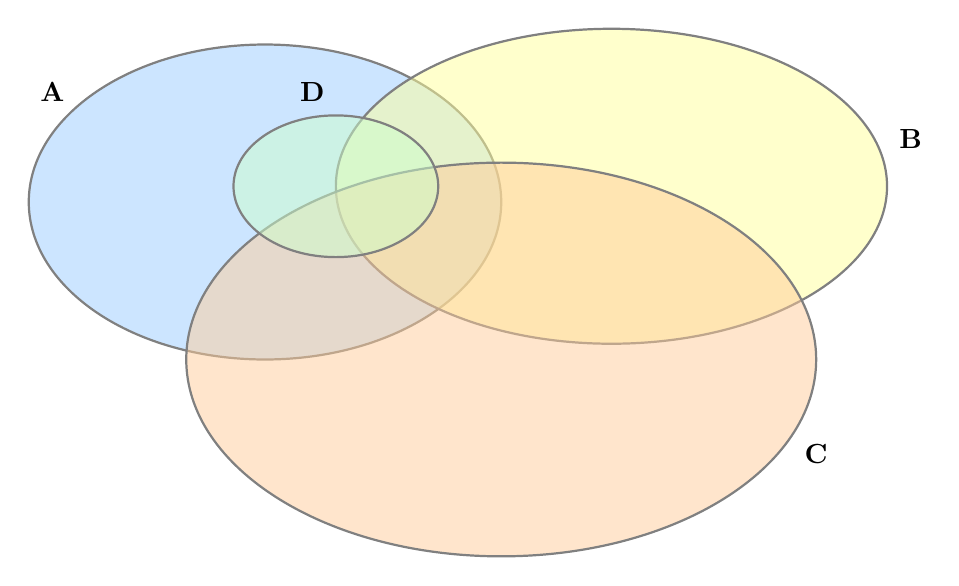
\begin{tikzpicture}
	    \definecolor{myblue}{rgb}{0.6,0.8,1.0}
	\definecolor{myyellow}{rgb}{1.0,1.0,0.6}
	\definecolor{myorange}{rgb}{1.0,0.8,0.6}
	\definecolor{mygreen}{rgb}{0.8,1.0,0.8}
	
	% A (blau)
	\filldraw[thick, gray, fill=myblue, fill opacity=0.5] (-3,0) ellipse (3cm and 2cm);
	\node at (-5.7,1.4) {\textbf{A}};
	
	% B (gelb)
	\draw[thick, gray, fill=myyellow, fill opacity=0.5] (1.4,0.2) ellipse (3.5cm and 2cm);
	\node at (5.2,0.8) {\textbf{B}};
	
	% C (orange)
	\filldraw[thick, gray, fill=myorange, fill opacity=0.5] (0,-2) ellipse (4cm and 2.5cm);
	\node at (4,-3.2) {\textbf{C}};
	
	% D (grün)
	\draw[thick, gray, fill=mygreen, fill opacity=0.5] (-2.1,0.2) ellipse (1.3cm and .9cm);
	\node at (-2.4,1.4) {\textbf{D}};
\end{tikzpicture}
\end{center}


\textbf{Aufgabe 2 (Ich spring im Dreieck):} Wie hängen die folgenden Mengen zusammen?
Stellt eure Überlegungen graphisch mit Hilfe eines Mengen-Diagramms dar!

\begin{itemize}
\item die Menge aller gleichschenkligen Dreiecke
\item die Menge aller Dreiecke
\item die Menge aller gleichseitigen Dreiecke
\item die Menge aller rechtwinkligen Dreiecke
\item die Menge aller gleichwinklingen Dreiecke
\end{itemize}

\vspace*{10mm}
%\newpage
\printlicense

\printsocials

\end{document}
